\chapter{Implementation}
\section{Introduction}
Initially, when starting the development of this model, we looked at various tools and options to implement the model in code.  We settled on using Jupyter Notebooks along with a number of libraries to help make the development of this model easier and faster.  The useful thing about Jupyter Notebooks is that they can be opened in a browser and all the code can be run from a single page.  We will detail the development of this model both in this thesis and include notes in the notebook itself to explain my rationale behind implementing the model in a certain way.  During the initial phase of implementation, I used both the Keras documentation \cite{keras} and Tensorflow documentation \cite{tensorflow} as references to ensure that the model's development was following standard practices and to ensure that the model was optimized to allow training in a timely manner. 
\\
Due to the limited support for AMD graphics cards(currently I use a 6700XT which does not have RoCM support\cite{amdLimitations}) in a variety of popular AI frameworks/libraries at the time of my writing this thesis, we decided it was best to use Google Colab Pro when training both the CNNs and the GANs this may offer some limitations in terms of memory and computational power.  Google Colab Pro, however, does offer a lot of advantages when it comes to quickly setting up an environment in which to train these models, it is for this reason that I have chosen to use it for training the models.
\\
For the purpose of reproducible results, we included the following lines of code np.random.seed(9) and set the random seed of Keras to 10 so that other researchers can reproduce the results and build upon this study.  All the datasets are loaded and split using a seed of 1337 also so that the train/test split is the exact same every time.
\section{CNN Baseline Model Design and Comparison}
When starting the implementation phase, we decided to use the following resource to develop baseline CNN models\cite{imageClassificationKeras}.  We plan on modifying this resource to achieve a relatively high training/validation accuracy when training on the original dataset.  We plan on using these models to get a metric with which we can compare models generated on the original dataset to the models which are generated on the synthetic dataset.  It is in this way we can accurately compare the effects of the synthetic dataset on the accuracy of the implemented models.
\\
After this initial comparison is done with the models trained on the original dataset versus the models trained on the synthetic dataset.  We then plan on focusing on which architectures would work best when developing the CNN and how the models trained on the synthetic dataset can be improved.
\\
To start I decided to use the following settings when developing a CNN to be used when training on the x-ray COVID-19 dataset.  This dataset is made up of images that are labeled either 1 or 0 with 1 being COVID-positive and 0 being COVID-negative.  I have included the architecture of the layers of the model in the table below\ref{tab:First CNN baseline model architecture for X-ray COVID-19 dataset}
\begin{table}[H]
    \centering
    \resizebox{\textwidth}{!}{
    \begin{tabular}{|c|c|c|c|c|c|c|}
    \hline
        Layer Number 
        & Layer Type
        & Layer Size 
        & Kernel Size
        & Strides
        & Padding
        & Activation\\
        \hline
        1 & Conv2D Layer & 16 & (3,3) & 2 & Same & Swish\\
        2 & SeparableConv2D Layer & 32 & (3,3) & 2 & Same & Swish \\
        3  & SeparableConv2D Layer & 64 & (3,3) & 2 & Same & Swish \\
        4  & MaxPooling2D & 2 & 2 & None & Same & None \\
        5 & Residual & 128 & (3,3) & 2 & Same & Swish \\
        6 & SeparableConv2D & 256 & (3,3) & None & Same & Swish \\
        7 & GlobalAveragePooling2D & 1 & None & None & None & Sigmoid \\
        \hline
    \end{tabular}
    }
    \caption{First CNN baseline model architecture for X-ray COVID-19 dataset}
    \label{tab:First CNN baseline model architecture for X-ray COVID-19 dataset}
\end{table}
For the padding the keyword ''same'' means that the input is padded with 0s evenly, both up and down and left and right of the image. The input was also scaled to normalize the data using the following line of code ''1.0 / 255)(inputs)''  After each layer batch normalization was performed excluding the residual, max pooling, and global average pooling 2D layers.  The use of the activation function ``swish`` was chosen due to studies showing it's performance matched or outperformed ReLU for certain tasks\cite{swishAndRelu}. Swish differs slightly in comparison to ReLU in that there isn't a sharp rise as the weight approaches 0. 
 \begin{figure}[H]
    \centering
    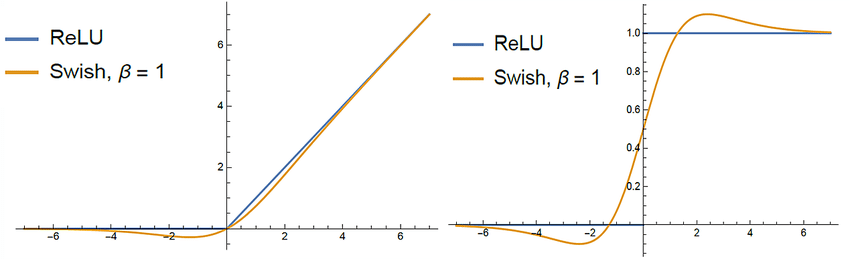
\includegraphics[width=1\textwidth,height=15cm,keepaspectratio]{Images/Swish ReLU activations.PNG}\\
    \caption{Figure of Swish and ReLU activation functions(Image courtesy of Madhura Ingalhalikar)\cite{swishReluDiagram}}
    \label{fig:Figure of Swish and ReLU activation functions}
\end{figure}
The model uses a dropout of 0, given the small size of the dataset I didn't want to drop neurons from the network.  The model was trained using a 70/30 training-validation split as I found this worked the best when training and testing the model. I also used the following settings when using model.compile() 
\begin{table}[H]
    \centering
    \resizebox{\textwidth}{!}{
    \begin{tabular}{|c|c|c|c|c|c|}
    \hline
         Optimizer
         & Loss Function 
         & Metric
         & Batch Size
         & Steps Per Epoch
         & Number of Epochs\\
         \hline
         Adam with a learning rate of $1e-3$ & Binary CrossEntropy & Accuracy & 16 & 1 & 9\\
         \hline
    \end{tabular}
    }
    \caption{First CNN baseline model hyperparameters for X-ray COVID-19 dataset}
    \label{tab:First CNN baseline model hyperparameters for X-ray COVID-19 dataset}
\end{table}
The model was trained for a total of 9 epochs with 1 step per epoch (again due to the limitations in the size of the dataset) and achieved the following results.

\begin{table}[H]
    \centering
    \begin{tabular}{|c|c|c|c|}
    \hline
         Training Loss
         & Training Accuracy 
         & Validation Loss
         & Validation Accuracy\\
         \hline
         0.5495  & 1.0000 & 0.6755 & 0.8393\\
         \hline
    \end{tabular}
    \caption{First CNN baseline model results for X-ray COVID-19 dataset}
    \label{tab:First CNN baseline model results for X-ray COVID-19 dataset}
\end{table}
 \begin{figure}[H]
    \centering
    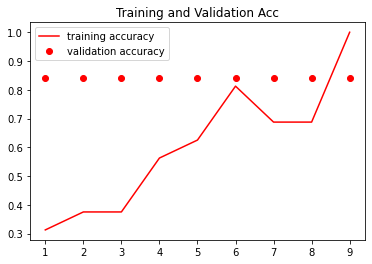
\includegraphics[width=1\textwidth,height=5cm,keepaspectratio]{Images/FirstCNNBaselineTrainAndValAcc.PNG}\\
    \caption{Figure of Train and Validation Accuracy of First CNN Baseline Model}
    \label{fig:First CNN Baseline Train and Validation Accuracy}
\end{figure}
 \begin{figure}[H]
    \centering
    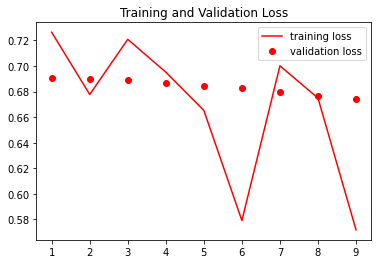
\includegraphics[width=1\textwidth,height=5cm,keepaspectratio]{Images/FirstCNNBaselineTrainAndValLoss.PNG}\\
    \caption{Figure of Train and Validation Loss of First CNN Baseline Model}
    \label{fig:First CNN Baseline Train and Validation Loss}
\end{figure}
As is shown from the results above\ref{tab:First CNN baseline model results for X-ray COVID-19 dataset} the model appears to overfit the training data which is to be expected given the small size of the dataset.  We can also see that the model has a reasonably high accuracy on the validation set but both the training set and the validation set have a high loss which is also caused by the small size of the dataset.
\\
After achieving relatively good performance on the X-ray COVID-19 dataset we then moved on to designing the model with the radiography dataset. This dataset is much larger than the original dataset, the radiography dataset contains a total of 30,306 image files broken into three classes.  In comparison, the X-ray COVID-19 dataset only contains 188 images belonging to two classes.  When designing this Convolutional network more thought had to be given to the split and which activation function to use for output, given that there are multiple classes.  When designing the CNN we decided to implement a much larger neural network given the amount of data available.  We tried using the initial network which was used for the X-ray COVID-19 dataset but the results were poor, increasing the size of the network led to better results.  When training the model I also found that a train/test split of 0.02 worked best using 98\% of the data to train and 2\% to test.
\begin{table}[H]
    \centering
    \resizebox{\textwidth}{!}{
    \begin{tabular}{|c|c|c|c|c|c|c|}
    \hline
        Layer Number 
        & Layer Type
        & Layer Size 
        & Kernel Size
        & Strides
        & Padding
        & Activation\\
        \hline
        1 & Conv2D Layer & 64 & (3,3) & 2 & Same & ReLU\\
        2 & SeparableConv2D Layer & 128 & (3,3) & 2 & Same & ReLU \\
        3  & SeparableConv2D Layer & 256 & (3,3) & 2 & Same & ReLU \\
        4 & SeparableConv2D Layer & 512 & (3,3) & 2 & Same & ReLU \\
        5 & SeparableConv2D Layer & 728 & (3,3) & 2 & Same & ReLU \\
        4  & MaxPooling2D & 3 & 2 & None & Same & None \\
        5 & Residual & 728 & (3,3) & 2 & Same & ReLU \\
        6 & SeparableConv2D & 1024 & (3,3) & None & Same & ReLU \\
        7 & GlobalAveragePooling2D & 3 & None & None & None & Softmax \\
        \hline
    \end{tabular}
    }
    \caption{Second CNN baseline model architecture for COVID Radiography Dataset}
    \label{tab:Second CNN baseline model architecture for COVID Radiography Dataset}
\end{table}


    \begin{table}[H]
    \centering
    \resizebox{\textwidth}{!}{
    \begin{tabular}{|c|c|c|c|c|c|}
    \hline
         Optimizer
         & Loss Function 
         & Metric
         & Batch Size
         & Steps Per Epoch
         & Number of Epochs\\
         \hline
         Adam with a learning rate of $1e-3$ & sparse categorical crossentropy & Accuracy & 32 & 18 & 50\\
         \hline
    \end{tabular}
    }
    \caption{Second CNN baseline model hyperparameters for COVID Radiography Dataset }
    \label{tab:Second CNN baseline model hyperparameters for COVID Radiography Dataset}
\end{table}
In this model we achieved a higher accuracy when using ReLU as opposed to swift the final results of the model are as follows:
\begin{table}[H]
    \centering
    \begin{tabular}{|c|c|c|c|}
    \hline
         Training Loss
         & Training Accuracy 
         & Validation Loss
         & Validation Accuracy\\
         \hline
         0.5146  & 0.7934 & 0.5743  & 0.7508\\
         \hline
    \end{tabular}
    \caption{Second CNN baseline results for COVID Radiography Dataset}
    \label{tab:Second CNN baseline results for COVID Radiography Dataset}
\end{table}
 \begin{figure}[H]
    \centering
    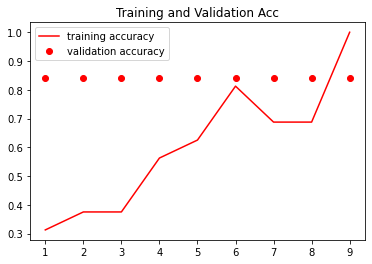
\includegraphics[width=1\textwidth,height=5cm,keepaspectratio]{Images/SecondCNNBaselineTrainAndValAcc.PNG}\\
    \caption{Figure of Train and Validation Accuracy of Second CNN Baseline Model}
    \label{fig:Second CNN Baseline Train and Validation Accuracy}
\end{figure}
 \begin{figure}[H]
    \centering
    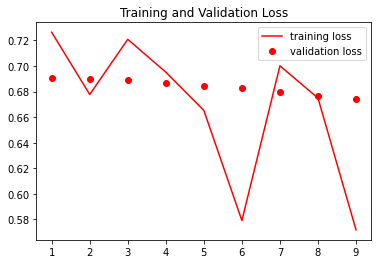
\includegraphics[width=1\textwidth,height=5cm,keepaspectratio]{Images/SecondCNNBaselineTrainAndValLoss.PNG}\\
    \caption{Figure of Train and Validation Loss of Second CNN Baseline Model}
    \label{fig:Second CNN Baseline Train and Validation Loss}
\end{figure}
As shown in the table\ref{tab:Second CNN baseline results for COVID Radiography Dataset} above we can see that the model has worse results when compared with the first baseline model.  The reason for this is due to a number of factors, one being the size of the dataset.  Given that this is a much larger dataset the model will have a more difficult time when classifying the images as there are now far more in the validation set when compared to the first model, there are 606 images for validation in this model as opposed to the 56 images in the first model.
\\
The third and final baseline CNN model was trained using the COVID-19 chest X-ray dataset. This dataset didn't have a standardised resolution for images so the images had to be resized which could possibly lead to lack of data quality and consistency when resized.  When training the model there was a high degree of loss which is to be expected given the data but this may be mitigated when generating images using a GAN which will be in a standardized resolution.  The model was trained with a train / test split of 80\% for the training set and 20\% for the test set.  The architecture of this model is as follows:
\begin{table}[H]
    \centering
    \resizebox{\textwidth}{!}{
    \begin{tabular}{|c|c|c|c|c|c|c|}
    \hline
        Layer Number 
        & Layer Type
        & Layer Size 
        & Kernel Size
        & Strides
        & Padding
        & Activation\\
        \hline
        1 & Conv2D Layer & 32 & (3,3) & 2 & Same & Swish\\
        2 & SeparableConv2D Layer & 64 & (3,3) & 2 & Same & Swish \\
        3  & MaxPooling2D & 11 & 2 & None & Same & None \\
        4 & Residual & 64 & (3,3) & 2 & Same & Swish \\
        5 & SeparableConv2D & 128 & (3,3) & None & Same & Swish \\
        6 & GlobalAveragePooling2D & 11 & None & None & None & Softmax \\
        \hline
    \end{tabular}
    }
    \caption{Third CNN baseline model architecture for COVID-19 Chest X-ray Dataset}
    \label{tab:Third CNN baseline model architecture for COVID-19 Chest X-ray Dataset}
\end{table}

    \begin{table}[H]
    \centering
    \resizebox{\textwidth}{!}{
    \begin{tabular}{|c|c|c|c|c|c|}
    \hline
         Optimizer
         & Loss Function 
         & Metric
         & Batch Size
         & Steps Per Epoch
         & Number of Epochs\\
         \hline
         Adam with a learning rate of $1e-3$ & categorical crossentropy & Accuracy & 10 & 1 & 10\\
         \hline
    \end{tabular}
    }
    \caption{Third CNN baseline model hyperparameters for COVID-19 Chest X-ray Dataset }
    \label{tab:Third CNN baseline model hyperparameters for COVID-19 Chest X-ray Dataset}
\end{table}
Due to the small size of the dataset the batch size was set to a low number. The steps per epoch and number of epochs were also relatively low when compared with the other datasets due to the limited amount of data present.  The model's performance is shown in the table below:
\begin{table}[H]
    \centering
    \begin{tabular}{|c|c|c|c|}
    \hline
         Training Loss
         & Training Accuracy 
         & Validation Loss
         & Validation Accuracy\\
         \hline
         1.6043  & 0.8125 & 2.2768 & 0.6714\\
         \hline
    \end{tabular}
    \caption{Third CNN baseline model results for COVID-19 Chest X-ray Dataset}
    \label{tab:Third CNN baseline model results for COVID-19 Chest X-ray Dataset}
\end{table}
 \begin{figure}[H]
    \centering
    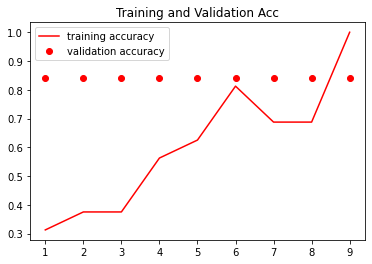
\includegraphics[width=1\textwidth,height=5cm,keepaspectratio]{Images/ThirdCNNBaselineTrainAndValAccBeforePreprocessing.png}\\
    \caption{Figure of Train and Validation Accuracy of Third CNN Baseline Model(Before Image Standardisation)}
    \label{fig:Third CNN Baseline Train and Validation Accuracy(Before Image Standardisation)}
\end{figure}
 \begin{figure}[H]
    \centering
    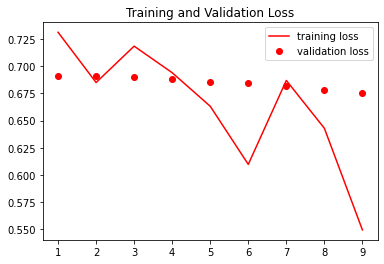
\includegraphics[width=1\textwidth,height=5cm,keepaspectratio]{Images/ThirdCNNBaselineTrainAndValLossBeforePreprocessing.png}\\
    \caption{Figure of Train and Validation Loss of Third CNN Baseline Model(Before Image Standardisation)}
    \label{fig:Third CNN Baseline Train and Validation Loss(before Pre-processing}
\end{figure}
As shown in the table above \ref{tab:Third CNN baseline model results for COVID-19 Chest X-ray Dataset} the model has a high degree of loss and the accuracy isn't very good on either the training or the test set.  This is to be expected as resizing the images when inputting them into the model will distort the information present.  The use of GANs to generate the data in a standardised resolution may help to mitigate this issue but as shown in the baseline model the lack of a uniform resolution for the images has led to poor performance.
\section{GAN Baseline Design and Comparison}
\subsection{GANs for Radiography Dataset}
Due to a large imbalance between classes in the dataset I decided to explore the use of GANs to create synthetic data for both the COVID positive images which comprise 7,232 images in this dataset and the Pneumonia positive images which comprise 2,690 images.  The normal class(healthy patients) is very over-represented in the data as it is comprised of 20,384 images, due to this imbalance the CNNs trained from this dataset will be heavily biased towards identifying the normal patients.  For this reason I have chose to use a number of Generative Adversarial Architectures to synthetically augment the classes lacking in data to balance the dataset and increase the generalization and robustness of the CNN models.
\subsection{VAE(Variational Auto Encoder)}
\subsubsection{COVID-19 Class Augmentation}
\subsubsection{Pneumonia Class Augmentation}

\subsection{DCGAN(Deep Convolutional GAN Network)}
\subsubsection{COVID-19 Class Augmentation}
When designing the DCGAN I experimented with a number of architectures, some of these architectures led to the GAN only producing black squares which was a sign of mode collapse.  Mode collapse occurs when the discriminator gets stuck at a local minimum and the generator learns to only produce the same type of image over and over again to fool the discriminator. I found switching from an ADAM optimizer to RMSPROP and experimenting with the learning rate and momentum led to far better results.  The model produced some promising results but a few of the X-Rays didn't appear to be the best of quality.  The lack of data was a challenge when training the DCGAN model as I only had 7,232 images to train with including the masks.    The following architecture was used to create the generator and discriminator:
\begin{minted}[linenos,tabsize=2,breaklines]{JavaScript}
discriminator = keras.Sequential(
    [
        keras.Input(shape=(128, 128, 3)),
        layers.Conv2D(64, kernel_size=4, strides=2, padding="same"),
        layers.LeakyReLU(alpha=0.5),
        layers.Conv2D(128, kernel_size=4, strides=2, padding="same"),
        layers.LeakyReLU(alpha=0.5),
        layers.Conv2D(128, kernel_size=4, strides=2, padding="same"),
        layers.LeakyReLU(alpha=0.5),
        layers.Flatten(),
        layers.Dropout(0.2),
        layers.Dense(1, activation="sigmoid"),
    ],
    name="discriminator",
)
discriminator.summary()

# Create the generator.
generator = keras.Sequential(
    [
        keras.Input(shape=(latent_dim,)),
        layers.Dense(8 * 8 * 128),
        layers.Reshape((8, 8, 128)),
        layers.Conv2DTranspose(256, kernel_size=4, strides=2, padding="same"),
        layers.LeakyReLU(alpha=0.2),
        layers.Conv2DTranspose(512, kernel_size=4, strides=2, padding="same"),
        layers.LeakyReLU(alpha=0.2),
        layers.Conv2DTranspose(1024, kernel_size=4, strides=2, padding="same"),
        layers.LeakyReLU(alpha=0.2),
        layers.Conv2DTranspose(64, kernel_size=4, strides=2, padding="same"),
        layers.LeakyReLU(alpha=0.2),
        layers.Conv2D(3, kernel_size=5, padding="same", activation="sigmoid"),
    ],
    name="generator",
)
generator.summary()
\end{minted}
The design of this GAN was based off of a Keras tutorial and the code was refactored for the purposes of this project\cite{DCGANKerasTutorial}.  The following hyper parameters were used when training the DCGAN model to generate synthetic COVID-19 X-Ray images: 
\begin{table}[H]
    \centering
    \resizebox{\textwidth}{!}{
    \begin{tabular}{|c|c|c|c|c|c|c|c|c|}
    \hline
         Generator Optimizer
         & Discriminator Optimizer 
         & Generator Learning Rate
         & Discriminator Learning Rate
         & Generator Momentum
         & Discriminator Momentum
         & Steps per Epoch
         & Batch Size
         & Number of Epochs\\
         \hline
         RMSPROP & RMSPROP & $1 \times 10 ^ -4$ & $1 \times 10 ^ -4$ & $1 \times 10 ^ -2$ & $1 \times 10 ^ -2$ & 1 & 16 & 452\\
         \hline
    \end{tabular}
    }
    \caption{DCGAN for Producing Synthetic Data From Radiography Dataset }
    \label{tab:DCGAN for Producing Synthetic Data From Radiography Dataset}
\end{table}
With this model architecture I was able to achieve a final score of 0.6094\% for the discriminator and 0.8001\% for the generator.
% include example images here produced from this GAN
\subsubsection{Pneumonia Class Augmentation}
The training of the DCGAN for the Pneumonia class took a lot of trial and error when training the GAN, as there is far less training data available for this class in comparison to the COVID class.  The Pneumonia class contains 2690 images of both the X-Rays and their masks, the COVID class contained 7,232 images for comparison which amounts to 4,542 more images.  It is clear to see the imbalance in this dataset given the difference between the various classes of which it is comprised.   During the training of this DCGAN I experimented with multiple hyper-parameters and trained many different GAN models.
\subsection{GANs for Chest X-Ray Dataset}
\subsection{GANs for X-Ray Dataset COVID-19}

\section{Improving CNN Models}
\section{Improving GAN Models}
\section{GANs in Conjunction}
\section{Conclusion}


